\documentclass{article}
\usepackage[utf8]{inputenc}
\usepackage[margin = 0.8in]{geometry}
\usepackage{graphicx}
\usepackage{amsmath, amssymb}
\usepackage{subcaption}
\usepackage{multirow}
\usepackage{mathtools}
\usepackage{float}


\title{CS534 - HW 1}
\author{Keith Chester}
\date{Due date: June 12 2022}

\begin{document}
\maketitle

\section*{Problem 2}
Suppose that two friends live in different cities within the map provided from our textbook Figure 3.1, presented below.

\begin{figure}[H]
    \centering
    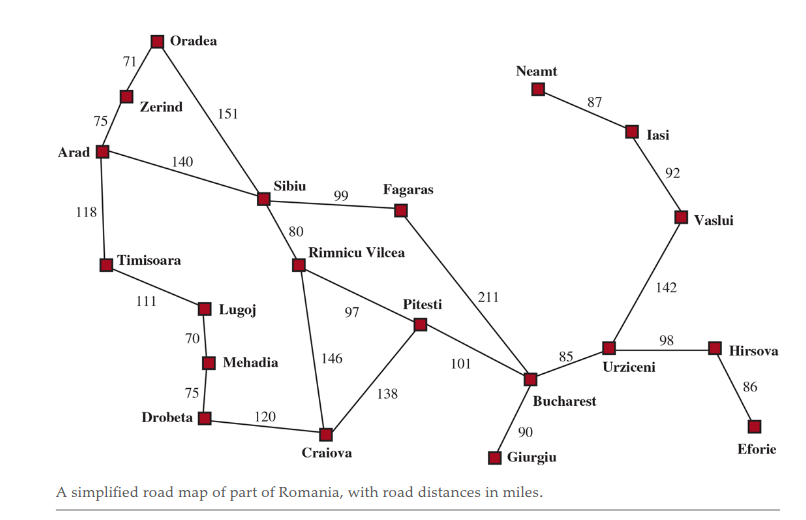
\includegraphics[width = 0.65\textwidth]{imgs/figure31.png}
    \label{fig:fig31}
\end{figure}

The amount of time needed to move from city $i$ to neighbor $j$ is equal to the road distance $D(i,j)$ between the cities. On each turn the friend that arrives first must wait until the other arrives before the next turn of travel can begin. Thus we are limited to the travel time of the slowest agent. We aim to get these friends to meet as quickly as possible.

\subsection*{1. Detailed Problem Formulation}
For our problem, we have two friends - $f_1$ and $f_2$. We wish to find a path such that both end up in the same city $c_{goal}$, at the same time, in the lowest possible time $t$. We have a cost between cities, a distance defined by $D(i,j)$ where $i$ and $j$ are adjacent cities. A given state is defined as $c_{f_1}$ and $c_{f_2}$, which is the city for each given friend. A given action on each discrete step is each friend moving to a new $c_{f_{1/2}}$ until they equal eachother.

\subsection*{2.Which heuristic functions are admissible?}
Suppose that $D(i, j)$ is the straight line distance between cities $i$ and $j$. Which of the following heuristic functions are admissibile?

\begin{itemize}
    \item $D(i,j)$
    \item $2D(i,j)$
    \item $\frac{D(i,j)}{2}$
\end{itemize}

\noindent To be admissible, the heuristic must not overestimate the actual cost of a given transition. Thus the second option, $2D(i,j)$, would not be admissible. The first and third options, $D(i,j)$ and $\frac{D(i,j)}{2}$, respectively, would be admissible.

\subsection*{3. Can a completely connected map have no solutions?}
Yes - since both travelers must travel at the same time, it's possible that a fully connected graph, such as a simple two node map. As both leave for the other's city, they find themselves in opposite cities again. This repeats forever.

\subsection*{4. Are there maps which every solution would require revisting a city?}
Yes. Consider a map with a singular path, with a cycle on the far end, to the side of the second friend's starting position. For example:

\begin{figure}[H]
    \centering
    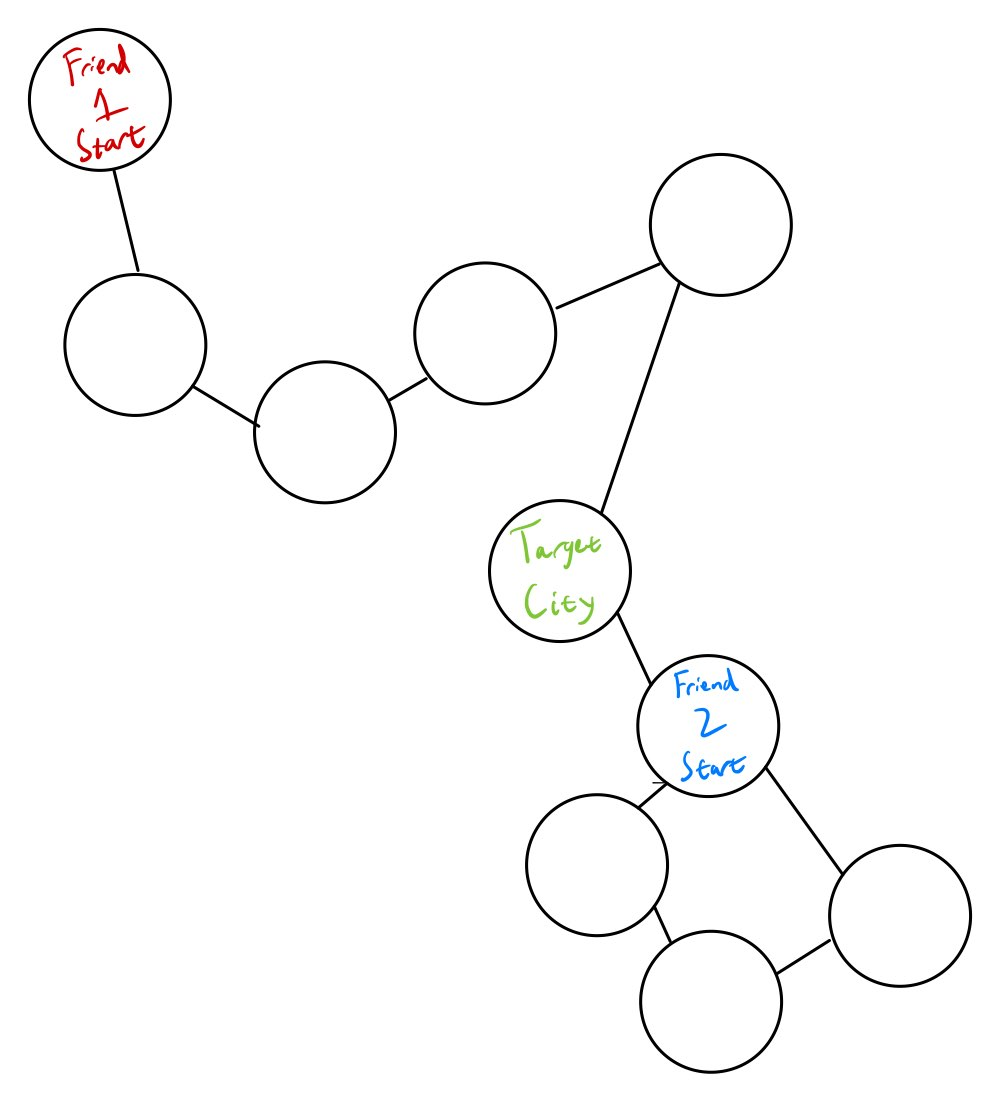
\includegraphics[width = 0.65\textwidth]{imgs/grid_example.jpg}
\end{figure}

\section*{Problem 3}

In this problem we explore a simple hill climbing agent and a genetic algorithm client.

\subsection*{Part C}

Here we compare the performance and utilization of the hill climbing agent and the genetic algorithm agent we built.

\begin{center}
    \begin{tabular}{ l c c c }
         Agent &     Generations &     Time to solution &    Fitness of solution \\ 
        Hill Climbing & --- &   6.19 seconds &        4669.4 meters \\  
        Genetic Algorithm & 1000  & 36.58 seconds  &      4074.4 meters  \\
        Genetic Algoirthm & 100 & 6.06 seconds & 4335.3 meters \\
    \end{tabular}
\end{center}

Here we see that while the hill climbing algorithm is significanlty quicker, just approximately 6 seconds to the genetic algorithm's 30+ - but the hill climbing algorithm gets stuck on a local minimum whereas the genetic algorithm continues to improve. If we drastically lower the number of generations we intend to utilize for the genetic algorithm, we get faster - faster even than hill climbing - and can occasionally score a better result still! Since the genetic algorithm has mutation and crossover causing high exploration, it does not get stuck as easily at suboptimal local minimums.

\section*{Problem 4}

\end{document}